% Creating a simple Title Page in Beamer
\documentclass[aspectratio=169,10pt,english,dvipsnames]{beamer}

% Pacotes
\usepackage{lipsum}
\usepackage{graphicx}
\usepackage{color}
\usepackage[table]{xcolor}
\usepackage{tikz}
\usepackage{tcolorbox}
\usepackage{amsmath}
\usepackage{amsfonts}
\usepackage{amssymb}
\usepackage{mathrsfs}
\usepackage{mathtools}
\usepackage{enumitem} 
\usepackage{float}
\usepackage[utf8]{inputenc}	

\usepackage{caption}

\usepackage[spanish, es-tabla]{babel}
\usepackage[babel, spanish=spanish]{csquotes}
\AtBeginEnvironment{quote}{\small}
\decimalpoint

\usetikzlibrary{decorations.pathreplacing,calc}
\usetikzlibrary{shadows}
\usetikzlibrary{positioning}

\usepackage{booktabs}

\usepackage{subcaption}

\usepackage{multicol}

\usepackage{multirow}


% Theme choice:
\usetheme{CambridgeUS}

% Cores personalizadas
\definecolor{PROFMATgreen}{RGB}{0, 138, 163}
\definecolor{UFTgreen}{RGB}{0, 137, 124}
\definecolor{UFTblue}{RGB}{0, 84, 132}
\definecolor{UFTyellow}{RGB}{253, 185, 46}
\definecolor{UFTgray}{RGB}{132, 134, 136}

\definecolor{UC}{RGB}{0,178,169}

% Ativar numeração de tabelas
\setbeamertemplate{caption}[numbered]

% Definir novo estilo de item com quadrado verde
\setlist[itemize,1]{label=\textcolor{UFTgreen}{\rule{1ex}{1ex}}}

\setbeamercolor*{structure}{bg=UFTgreen,fg=black}

\setbeamercolor*{palette primary}{fg=black,bg=PROFMATgreen}
\setbeamercolor*{palette secondary}{fg=white,bg=UFTblue}
\setbeamercolor*{palette tertiary}{fg=black,bg=UFTgreen}
\setbeamercolor*{palette quaternary}{fg=white,bg=black}

\setbeamercolor{section in toc}{fg=black,bg=white}
\setbeamercolor{alerted text}{fg=white}

\setbeamercolor*{item}{fg=PROFMATgreen}

\setbeamercolor{block title}{bg=UFTgreen,fg=white}
\setbeamercolor{block body}{bg=UFTgray!10,fg=black}

\setbeamercolor{titlelike}{fg=white, bg=UFTblue}
\setbeamercolor{frametitle}{bg=UFTgray!20,fg=UFTgreen}



\setbeamertemplate{background}{
    \parbox[c][\paperheight][c]{\paperwidth}{
        \vfill
        
\includegraphics[width=\paperwidth,height=\paperheight,keepaspectratio]{img/modelo/bakcground.png} 
        \vfill
    }
}


% Personalizar portada
\setbeamertemplate{title page}{
  \begin{columns}[c,totalwidth=\paperwidth]
    \column{.05\paperwidth}
      \centering
      \raisebox{0.1cm}{%
        \parbox{.5\paperwidth}{\centering\scriptsize
        Convocatoria 2023\\ «Proyectos de Generación de Conocimiento» y actuaciones\\ para la formación de personal investigador predoctoral\\ asociadas a dichos proyectos.}
      }
    \column{.45\paperwidth}
      \centering
      
\includegraphics[height=1.2cm]{img/UC_LogotipoPrincipal.png}
\end{columns}

  \vskip1em
  \begingroup
    \centering
    \begin{beamercolorbox}[sep=8pt,center,shadow=true,rounded=false]{title}
      \usebeamerfont{title}\inserttitle\par%
      \ifx\insertsubtitle\@empty\else
        \vskip0.25em{\usebeamerfont{subtitle}\usebeamercolor[fg]{subtitle}\insertsubtitle\par}%
      \fi
    \end{beamercolorbox}
    \vskip1em
    \begin{beamercolorbox}[sep=6pt,center]{author}\usebeamerfont{author}\insertauthor\end{beamercolorbox}
    \vskip0.2em
    \begin{beamercolorbox}[sep=5pt,center]{advisor}\usebeamerfont{institute}\advisorname\end{beamercolorbox}
    \vskip0.2em
    \begin{beamercolorbox}[sep=5pt,center]{institute}\usebeamerfont{institute}\insertinstitute\end{beamercolorbox}
    \vskip0.2em
    \begin{beamercolorbox}[sep=5pt,center]{date}\usebeamerfont{institute}\insertdate\end{beamercolorbox}
    \vskip0.5em
  \endgroup
  \vfill
}



% Remover bordas arredondadas dos blocks
\makeatletter
\setbeamertemplate{blocks}[default] % Isso remove o arredondamento
\makeatother


% Pacotes de citações
% ---

\usepackage[alf,abnt-etal-text=it,abnt-repeated-author-omit=yes,abnt-etal-list=0,abnt-etal-cite=3,abnt-emphasize=bf]{abntex2cite}	% Citações padrão ABNT



\setbeamercolor{bibliography entry author}{fg=black}
\setbeamertemplate{bibliography item}{\newblock}


\setbeamertemplate{frametitle continuation}{}

% Redefinir o separador para um traço
% Redefinir o separador
\captionsetup[figure]{labelformat=simple, labelsep=endash, textformat=period, font=footnotesize}
\captionsetup[table]{labelformat=simple, labelsep=endash, textformat=period, font=footnotesize}


% Redefine espaçamento antes e depois da legenda em figuras e tabelas
\captionsetup[figure]{aboveskip=2pt, belowskip=0pt}
\captionsetup[table]{aboveskip=2pt, belowskip=0pt}


% Define uma penalidade alta para a hifenização
\hyphenpenalty=10000
\tolerance=10000


% Personalizando o estilo da tabela de conteúdos
\setbeamertemplate{section in toc}[sections numbered]
\renewcommand{\thesection}{\textcolor{PROFMATgreen}{\arabic{section}}}
\renewcommand{\thesubsection}{\textcolor{PROFMATgreen}{\arabic{section}.\arabic{subsection}}}

\setbeamersize{text margin left=0.8cm, text margin right=0.8cm}


% Información
\title[HAMELIN: Human-Guided AutoML]{HAMELIN: Human-guided Automated Machine Learning\\ for Clinical Studies}
\author[Rafael Duque]{Rafael Duque}
\institute[UC]{Universidad de Cantabria}
\date{January 2026}

% Nombre del director
\newcommand{\advisorname}{\textbf{Advisor:}  Rafael Duque}

\begin{document}

% Slide (frame) del título
\begin{frame}
    \titlepage
\end{frame}


% Índice
\begin{frame}[t]
    \frametitle{Contents}
    \tableofcontents
\end{frame}

% Sección: Introduction
\section{Introduction}

\begin{frame}{Research Context}
    \begin{minipage}{0.55\textwidth}
        \begin{itemize}
            \item \textbf{AutoML democratization}:\\
            Rapid expansion of ML applications created strong need for tools reducing technical barriers
            
            \item \textbf{Gap in clinical research}:\\
            Existing AutoML tools ignore semantic hierarchy and temporal structure of clinical data
            
            \item \textbf{Human-Centered AI paradigm}:\\
            AI should amplify and empower humans, not replace them
            
            \item \textbf{HAMELIN proposal}:\\
            Human-Guided ML system designed specifically for Clinical Research Professionals (CRPs)
        \end{itemize}
    \end{minipage}%
    \begin{minipage}{0.45\textwidth}
        \centering
        \scriptsize
        \begin{block}{Key Challenges}
            \begin{itemize}
                \item Protocol-aware data organization
                \item Temporal structure handling
                \item Clinical missing data strategies
                \item Inclusion/exclusion logic
                \item Interpretability requirements
            \end{itemize}
        \end{block}
        
        \vspace{5mm}
        
        \begin{block}{Project Goals}
            End-to-end HGML software system for non-AI specialists in clinical research
        \end{block}
    \end{minipage}
\end{frame}


% Sección: State of the Art
\section{State of the Art}

\begin{frame}{AutoML Tools Landscape}
    \begin{block}{Commercial Tools}
        \textbf{Cloud providers}: Google AutoML, Azure Automated ML, AWS SageMaker Autopilot\\
        \textbf{Specialized platforms}: DataRobot, H2O Driverless AI, IBM Watson AutoAI
        
        \textbf{Limitation}: High licensing and infrastructure costs
    \end{block}
    
    \begin{block}{Free Tools Categories}
        \begin{multicols}{2}
            \begin{itemize}
                \item \textbf{Data integration}: MindsDB
                \item \textbf{Time-series}: Prophet
                \item \textbf{Hyperparameter optimization}: Optuna, Hyperopt, NNI
                \item \textbf{Pipeline automation}: PyCaret, AutoGluon, TPOT, Ludwig
                \item \textbf{Neural architecture}: AutoKeras
                \item \textbf{Feature engineering}: Featuretools
            \end{itemize}
        \end{multicols}
    \end{block}
    
    \textbf{Key finding}: Most tools prioritize performance over usability, interpretability and human control
\end{frame}

\begin{frame}{Human-Centered AI Framework}
    \begin{minipage}{0.5\textwidth}
        \begin{itemize}
            \item \textbf{Paradigm shift}:\\
            Decoupling automation from human control
            
            \item \textbf{Two-dimensional conception}:\\
            High automation + High human control simultaneously
            
            \item \textbf{Goal}:\\
            Upper-right quadrant: systems with extensive automation yet meaningful user control
            
            \item \textbf{Applied to AutoML}:\\
            13 free tools analyzed according to HCAI dimensions
        \end{itemize}
    \end{minipage}%
    \begin{minipage}{0.5\textwidth}
        \centering
        \begin{tikzpicture}[scale=0.65, transform shape]
            \draw[->, thick] (0,0) -- (8,0) node[anchor=north, xshift=-1.5cm] {\scriptsize Computer Automation};
            \draw[->, thick] (0,0) -- (0,8) node[anchor=south east, rotate=90] {\scriptsize Human Control};
            \draw[dashed] (0,4) -- (8,4);
            \draw[dashed] (4,0) -- (4,8);
            \node[align=center, font=\tiny] at (2,2) {Low \\ Human Control \\ Low \\ Automation};
            \node[align=center, font=\tiny] at (6,2) {Low \\ Human Control \\ High \\ Automation};
            \node[align=center, font=\tiny] at (2,6) {High \\ Human Control \\ Low \\ Automation};
            \node[align=center, font=\tiny, fill=green!20] at (6,6) {\textbf{HCAI Goal} \\ High \\ Human Control \\ High \\ Automation};
        \end{tikzpicture}
        
        \vspace{3mm}
        
        \scriptsize
        \textbf{Result}: No tool achieves maximum on both dimensions simultaneously
    \end{minipage}
\end{frame}

\begin{frame}{HCAI Framework Applied to AutoML Tools}
    \begin{table}[ht]
        \centering
        \tiny
        \renewcommand{\arraystretch}{1.2}
        \resizebox{\textwidth}{!}{%
        \begin{tabular}{c c c c | c c c c c c}
            \toprule
            \multirow{2}{*}{\textbf{Tool}} 
              & \multicolumn{3}{c|}{\textbf{Human Control}} 
              & \multicolumn{6}{c}{\textbf{Automation}} \\ \cmidrule(lr){2-4} \cmidrule(lr){5-10}
              & \textbf{Easy-to-use} 
              & \textbf{Configurable} 
              & \textbf{Interpretable} 
              & \textbf{Data types} 
              & \textbf{Cleaning} 
              & \textbf{Feature eng.} 
              & \textbf{Training} 
              & \textbf{Tuning} 
              & \textbf{Validation} \\ \midrule
            MindsDB & Medium & Low & Medium & \checkmark & \checkmark & \checkmark & \checkmark & \checkmark & \checkmark \\
            H2O-3 & Medium & High & Medium & \checkmark & \checkmark & \checkmark & \checkmark & \checkmark & \checkmark \\
            Ludwig & Medium & High & Medium & \checkmark & \checkmark & \checkmark & \checkmark & \checkmark & \checkmark \\
            PyCaret & Low & High & Medium & \checkmark & \checkmark & \checkmark & \checkmark & \checkmark & \checkmark \\
            AutoGluon & Medium & High & Medium & \checkmark & \checkmark & \checkmark & \checkmark & \checkmark & \checkmark \\
            TPOT & Low & High & Low & \checkmark &  & \checkmark & \checkmark & \checkmark & \checkmark \\
            AutoKeras & Low & High & Low &  &  &  & \checkmark & \checkmark & \checkmark \\
            Auto-Sklearn & Low & High & Low & \checkmark & \checkmark & \checkmark & \checkmark & \checkmark & \checkmark \\ 
            \bottomrule
        \end{tabular}}
    \end{table}
    
    \vspace{2mm}
    
    \begin{itemize}
        \item \textbf{Observation}: Tools like Ludwig, H2O-3, AutoGluon offer broad automation with moderate human control
        \item \textbf{Gap}: Limited interactivity and restricted opportunities for domain experts to guide the process
    \end{itemize}
\end{frame}

\begin{frame}{Human-Guided Machine Learning}
    \begin{block}{HGML Concept}
        Concrete realization of HCAI principles: systematic incorporation of expert knowledge into ML workflows
    \end{block}
    
    \begin{itemize}
        \item \textbf{Hybrid approach}: Automated search + Active expert guidance
        
        \item \textbf{Expert involvement throughout pipeline}:\\
        \begin{itemize}
            \item \textbf{Data level}: Feature/instance selection, quality control, domain constraints\\
            \item \textbf{Model development}: Algorithm selection, hyperparameter bounds, preprocessing strategies\\
            \item \textbf{Evaluation}: Custom metrics, sensitivity analysis, clinical interpretation
        \end{itemize}
        
        \item \textbf{Five core goals}:
        \begin{enumerate}
            \item High predictive performance
            \item Fast optimization
            \item Transparency and interpretability
            \item Customizability and flexibility
            \item Usability and rich interaction
        \end{enumerate}
    \end{itemize}
    
    \textbf{Challenge}: Most existing proposals only partially address the pipeline or lack practical software implementation
\end{frame}

\begin{frame}{HGML Approaches Comparison}
    \begin{table}[h]
        \centering
        \scriptsize
        \resizebox{\textwidth}{!}{%
        \begin{tabular}{lcccccccccccc}
            \toprule
            \multirow{2}{*}{\textbf{Reference}} &
            \multicolumn{3}{c}{\textbf{Data Use}} &
            \multicolumn{3}{c}{\textbf{Model Development}} &
            \multicolumn{3}{c}{\textbf{Model Interpretation}} &
            \multirow{2}{*}{\textbf{Software}} &
            \multirow{2}{*}{\textbf{HCAI eval.}} \\ 
            \cmidrule(lr){2-4} \cmidrule(lr){5-7} \cmidrule(lr){8-10} &
            \textbf{Variable sel.} & 
            \textbf{Requirements} & 
            \textbf{Instance sel.} & 
            \textbf{Model sel.} & 
            \textbf{Parameters} & 
            \textbf{Design} & 
            \textbf{Assessment} & 
            \textbf{Comparison} & 
            \textbf{Param. comp.} & & \\ 
            \midrule
            Gil et al. (2019) & $\checkmark$ & $\checkmark$ & $\checkmark$ & $\checkmark$ & $\checkmark$ & $\checkmark$ & $\checkmark$ & $\checkmark$ & $\checkmark$ & -- & -- \\ 
            Francia et al. (2023) & $\checkmark$ & $\checkmark$ & -- & $\checkmark$ & $\checkmark$ & $\checkmark$ & $\checkmark$ & $\checkmark$ & -- & Expert-only & -- \\ 
            Lee et al. (2020) & $\checkmark$ & $\checkmark$ & $\checkmark$ & $\checkmark$ & $\checkmark$ & $\checkmark$ & $\checkmark$ & $\checkmark$ & $\checkmark$ & -- & -- \\ 
            Lindauer et al. (2024) & $\checkmark$ & $\checkmark$ & -- & $\checkmark$ & $\checkmark$ & $\checkmark$ & $\checkmark$ & $\checkmark$ & $\checkmark$ & -- & -- \\ 
            \textbf{HAMELIN} & $\checkmark$ & $\checkmark$ & $\checkmark$ & $\checkmark$ & $\checkmark$ & $\checkmark$ & $\checkmark$ & $\checkmark$ & $\checkmark$ & $\checkmark$ & $\checkmark$ \\ 
            \bottomrule
        \end{tabular}%
        }
    \end{table}
    
    \vspace{3mm}
    
    \begin{block}{HAMELIN Contribution}
        \textbf{Only approach} providing:
        \begin{itemize}
            \item End-to-end pipeline coverage
            \item Ready-to-use software implementation
            \item Evaluation based on HCAI criteria
            \item Design for non-AI specialists (CRPs)
        \end{itemize}
    \end{block}
\end{frame}


% Sección: CRP Competencies
\section{CRP Competencies Integration}

\begin{frame}{Clinical Research Professionals: Domain Expertise}
    \begin{itemize}
        \item \textbf{Protocol-aware data organization}:\\
        Distinguish demographics, clinical measurements, exposures, outcomes, inclusion/exclusion criteria\\
        Semantic hierarchy ignored by traditional AutoML
        
        \item \textbf{Temporal structure and protocol phases}:\\
        Screening → Baseline → Intervention → Follow-up → Endpoint\\
        Prevent data leakage using only information available at prediction time
        
        \item \textbf{Clinical missing data handling}:\\
        Missing Completely At Random, Missing At Random, Missing Not At Random\\
        Domain-specific strategies (safety variables, longitudinal measurements)
        
        \item \textbf{Inclusion/exclusion logic}:\\
        Complex criteria from study protocols\\
        Define analysis population (not just preprocessing)
        
        \item \textbf{Hypothesis-driven variable selection}:\\
        Clinical hypotheses grounded in prior research and pathophysiology
    \end{itemize}
\end{frame}

\begin{frame}{Design Process: From Protocols to Mockups}
    \begin{minipage}{0.48\textwidth}
        \begin{block}{Real Clinical Protocols Analyzed}
            \begin{itemize}
                \item \textbf{COLCHI-COVID}: Clinical trial (colchicine efficacy)
                \item \textbf{EPA-Registro COVID-19}: Patient registry
                \item \textbf{UPPS}: Observational study (pressure injuries in neurosurgery)
                \item \textbf{VACAB-2022}: Clinical trial (prosthesis infections)
            \end{itemize}
        \end{block}
        
        \vspace{3mm}
        
        \textbf{Iterative participatory design}:\\
        Mockups → CRP feedback → Refinement
    \end{minipage}%
    \hfill
    \begin{minipage}{0.48\textwidth}
        \begin{block}{Key CRP Feedback}
            \begin{itemize}
                \item Prefer clinical terminology (``primary variable'' vs ``target'')
                \item Need project metadata visibility
                \item Require flexible variable selection
                \item Request recruitment tracking
                \item Demand model transparency
                \item Want automatic ``Table 1'' generation
            \end{itemize}
        \end{block}
    \end{minipage}
\end{frame}

\begin{frame}{Mockups}
    \begin{figure}[h]
        \centering
        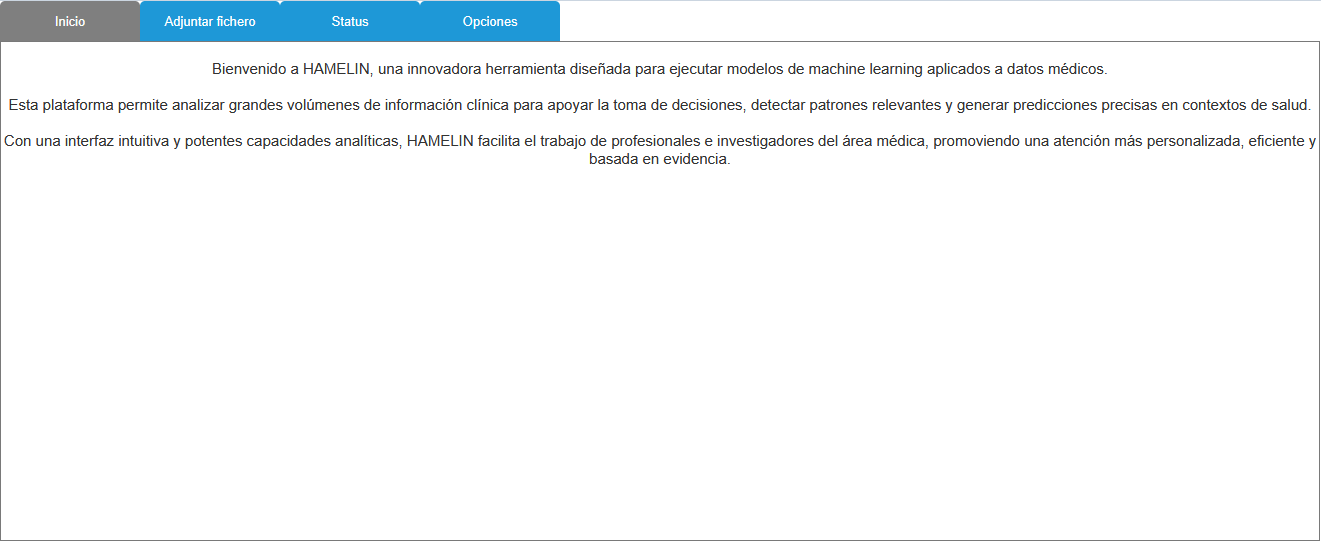
\includegraphics[width=0.8\textwidth]{img/Mockup/Mockup-Inicio.png}
    \end{figure}
\end{frame}

\begin{frame}{Mockups}
    \begin{figure}[h]
        \centering
        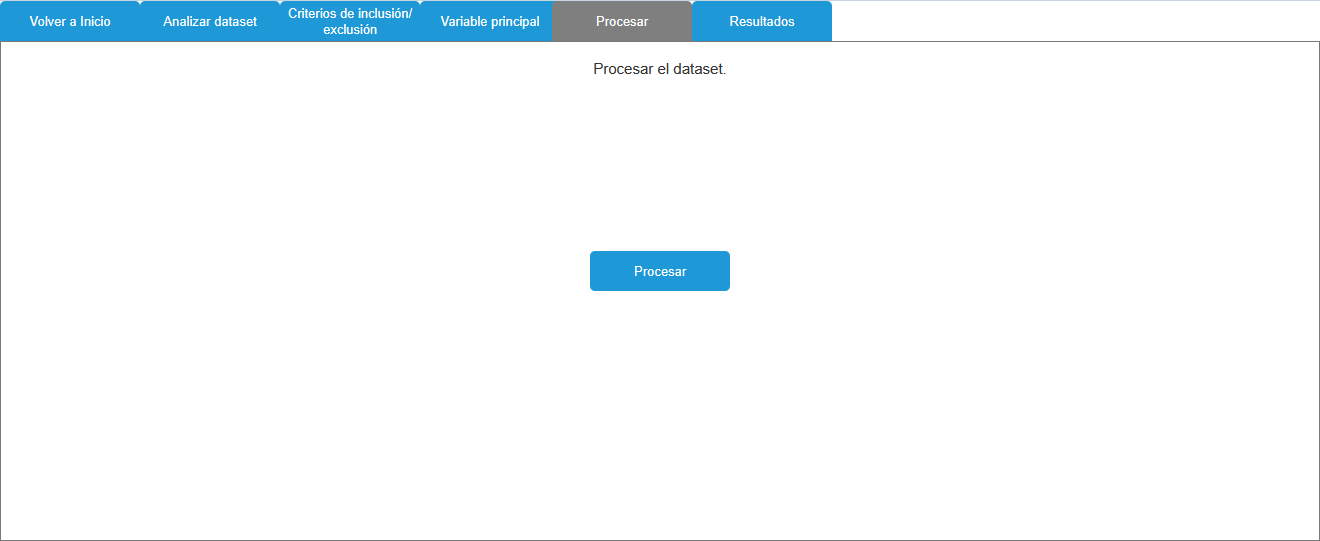
\includegraphics[width=0.8\textwidth]{img/Mockup/Mockup-Process.png}
        \end{figure}
\end{frame}

\begin{frame}{Mockups}
    \begin{figure}[h]
        \centering
        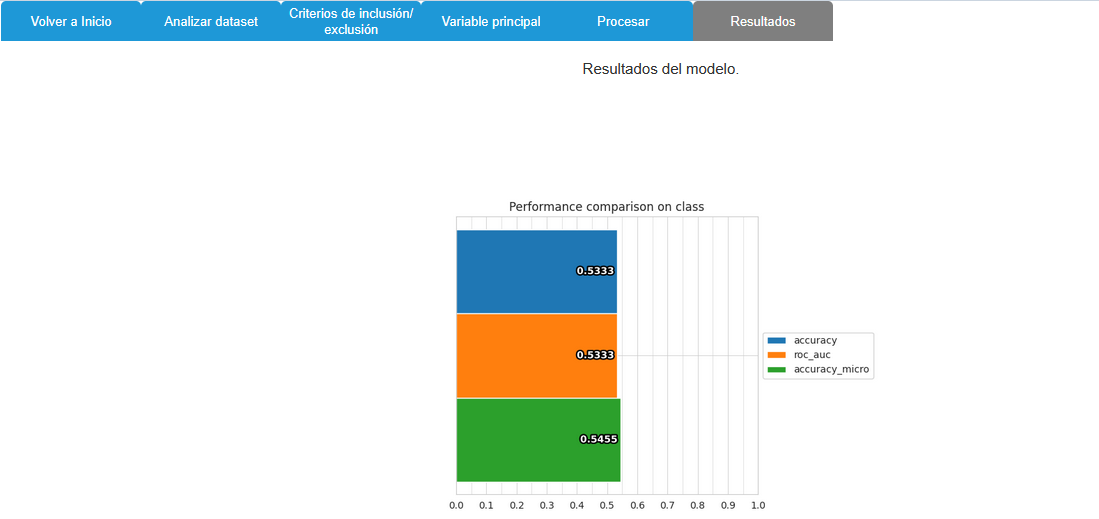
\includegraphics[width=0.8\textwidth]{img/Mockup/Mockup-Resultados.png}
        \end{figure}
\end{frame}


% Sección: HAMELIN System
\section{HAMELIN System}

\begin{frame}{System Architecture}
    \begin{figure}[H]
        \centering
        \scalebox{0.6}{
        \begin{tikzpicture}[
            node distance=2cm,
            box/.style={
                rectangle,
                draw,
                text width=4cm,
                text centered,
                minimum height=2cm,
                rounded corners=0.3cm,
                drop shadow,
                line width=1pt,
                font=\scriptsize
            },
            frontend/.style={box, fill=pink!35, draw=pink!70},
            backend/.style={box, fill=cyan!10, draw=cyan!50},
            ludwig/.style={box, fill=yellow!35, draw=yellow!70},
            arrow/.style={->, thick, color=gray!70, line width=0.8pt}
        ]
        
        \node[frontend] (frontend) at (0,0) {
            \textbf{Frontend}\\
            \textit{GUI}\\[2mm]
            Dataset loading/visualization\\
            Intuitive configuration\\
            Tab navigation\\
            Results presentation\\
            Input validation
        };
        \node[backend] (backend) at (5.5,0) {
            \textbf{Backend}\\
            \textit{Core Logic}\\[2mm]
            Data validation\\
            Command translation\\
            Config file generation\\
            Workflow coordination\\
            Error handling
        };
        \node[ludwig] (ludwig) at (11,0) {
            \textbf{Ludwig}\\
            \textit{AutoML Engine}\\[2mm]
            Model training\\
            Algorithm selection\\
            Performance evaluation\\
            Hyperparameter optimization\\
            Prediction
        };
        
        \draw[arrow] (frontend.east) -- (backend.west);
        \draw[arrow] (backend.west) -- (frontend.east);
        \draw[arrow] (backend.east) -- (ludwig.west);
        \draw[arrow] (ludwig.west) -- (backend.east);
        
        \node[above=0.8cm of frontend.north, 
              rectangle, 
              draw=gray!50, 
              fill=gray!10, 
              text width=2.5cm, 
              text centered,
              rounded corners=0.2cm] (user) {
            \scriptsize \textbf{User}\\
            \scriptsize Clinical researcher
        };
        \draw[arrow] (user.south) -- (frontend.north);
        \draw[arrow] (frontend.north) -- (user.south);
        
        \end{tikzpicture}
        }
    \end{figure}
    
    \begin{itemize}
        \item \textbf{Modular architecture}: Interface logic separated from AutoML engine
        \item \textbf{Technology stack}: Python, Qt Designer, Ludwig (v0.10.4), YAML configuration
        \item \textbf{Flexibility}: Ludwig module replaceable by other AutoML frameworks
    \end{itemize}
\end{frame}

\begin{frame}{Tab-Based Workflow}
    \begin{block}{Seven-Tab Pipeline}
        \begin{enumerate}
            \item \textbf{Start}: Project creation, metadata, dataset loading
            \item \textbf{Status}: Automatic exploration (descriptive statistics, missing data heatmap, recruitment timeline, Table 1)
            \item \textbf{Primary Variable}: Target selection, automatic task type detection (binary/multi-class/regression)
            \item \textbf{Criteria}: Inclusion/exclusion rule builder (AND/OR/NOT logic, real-time population filtering)
            \item \textbf{Settings}: Metrics selection, missing data strategies, time-dependent flag, runtime limit
            \item \textbf{Process}: Model training with real-time monitoring (progress bar, current/best model, ETA)
            \item \textbf{Results}: Performance presentation (confusion matrix, metrics table, feature importance)
        \end{enumerate}
    \end{block}
    
    \textbf{Key feature}: Iterative refinement — users can return to earlier tabs, modify choices, and re-train
\end{frame}

\begin{frame}{Interface}
    \begin{figure}[h]
        \centering
        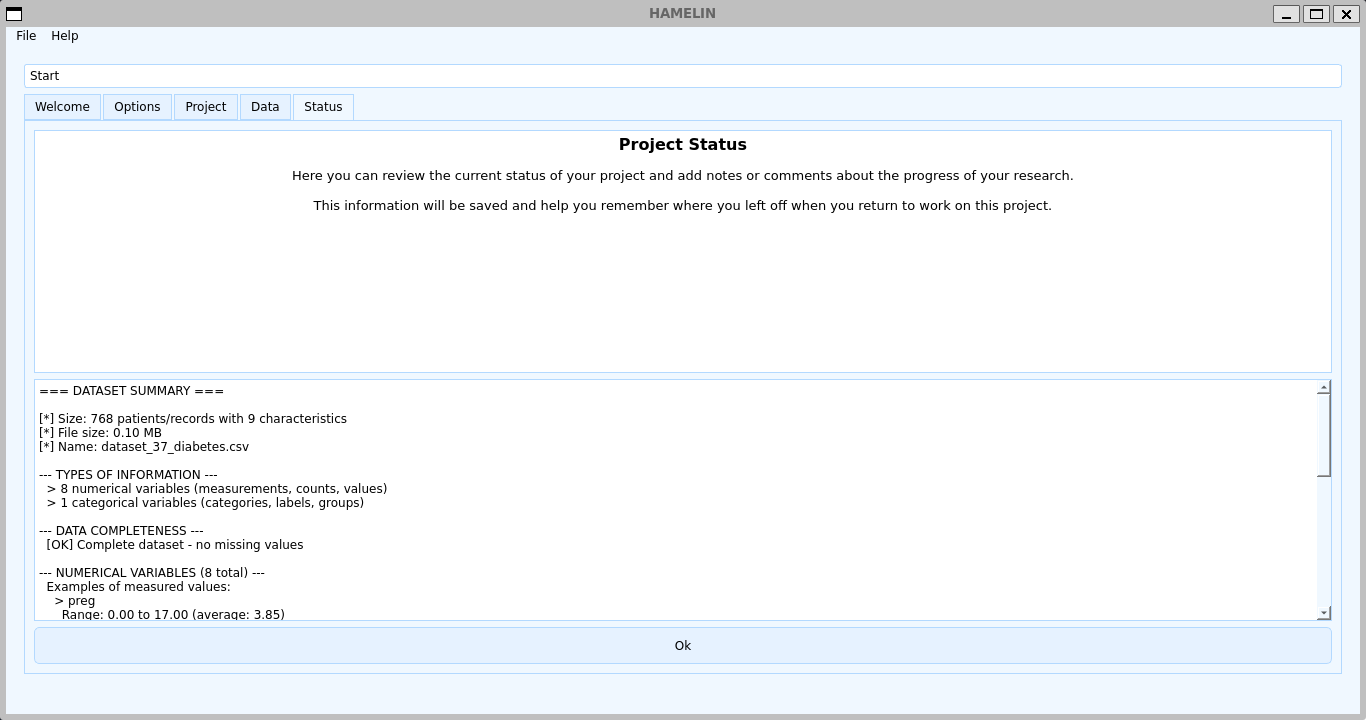
\includegraphics[width=0.8\textwidth]{img/Interface/interface-status.png}
    \end{figure}
\end{frame}

\begin{frame}{Interface}
    \begin{figure}[h]
        \centering
        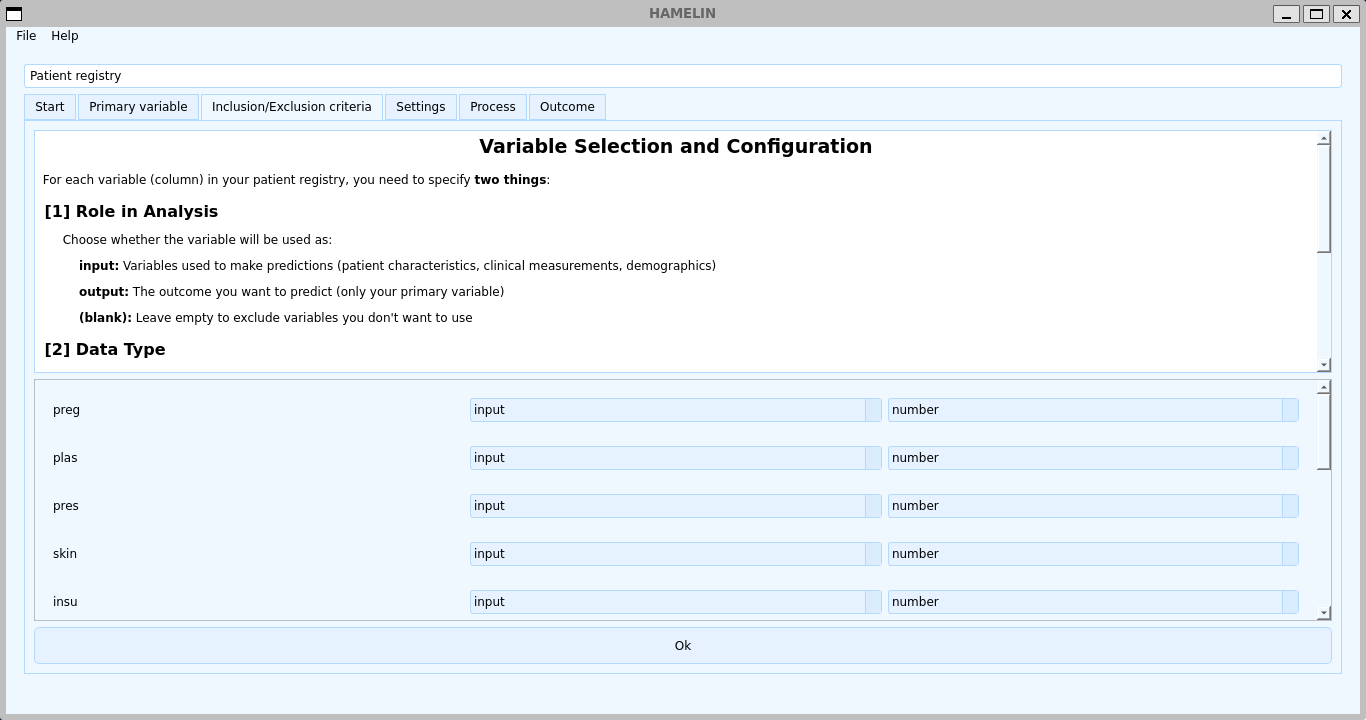
\includegraphics[width=0.8\textwidth]{img/Interface/interface-criteria.png}
    \end{figure}
\end{frame}

\begin{frame}{Interface}
    \begin{figure}[h]
        \centering
        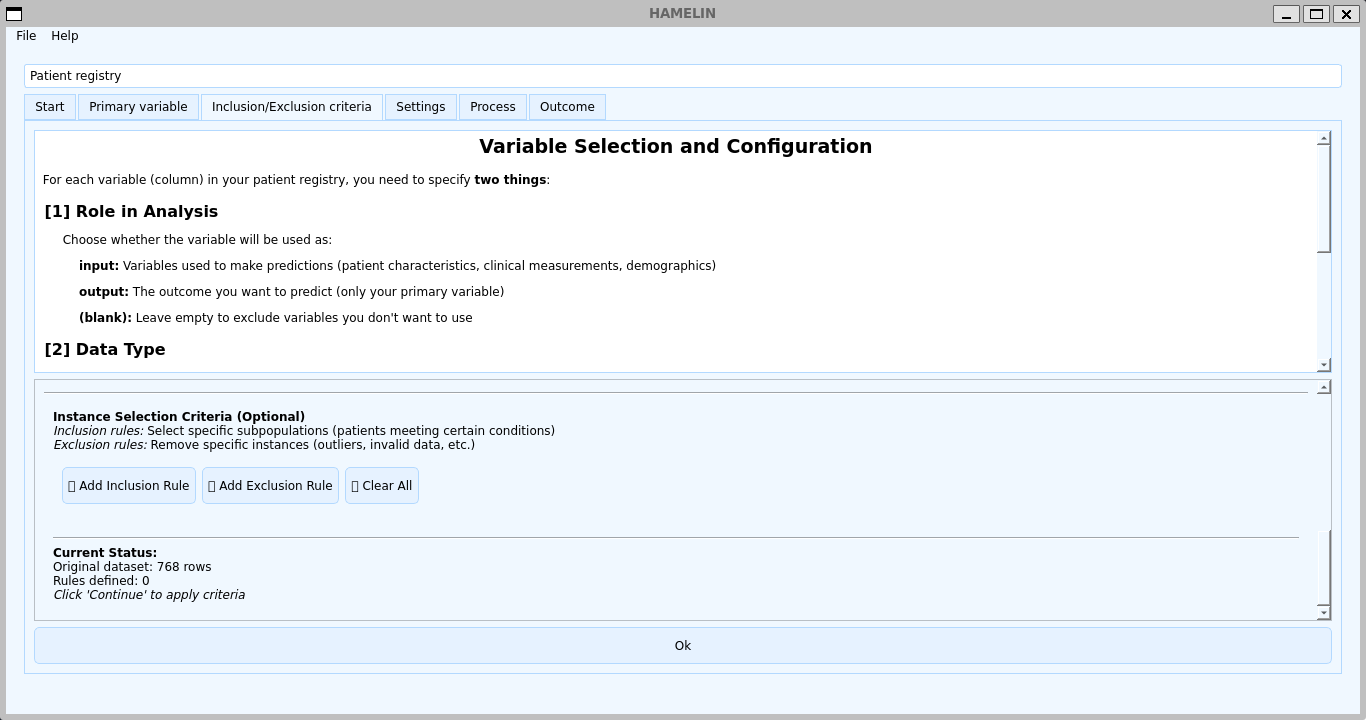
\includegraphics[width=0.8\textwidth]{img/Interface/interface-criteria2.png}
    \end{figure}
\end{frame}

\begin{frame}{Interface}
    \begin{figure}[h]
        \centering
        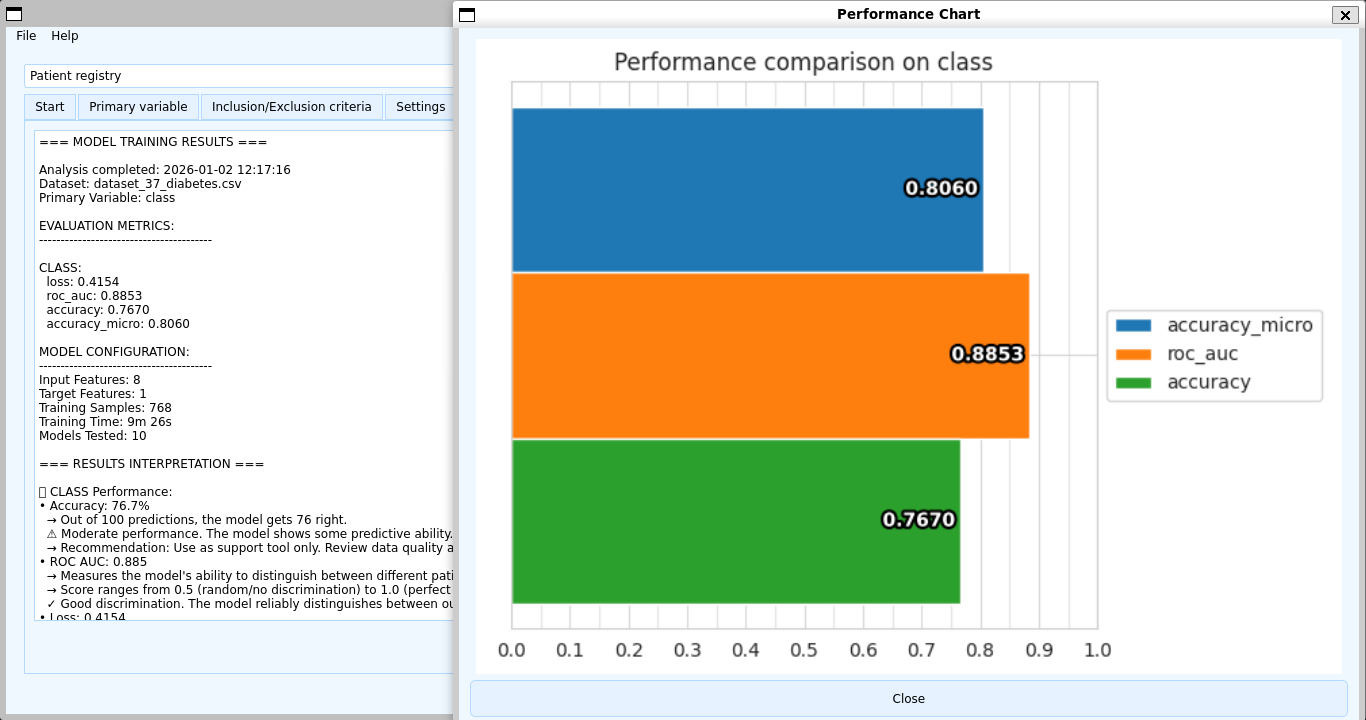
\includegraphics[width=0.8\textwidth]{img/Interface/interface-performance.png}
    \end{figure}
\end{frame}

\begin{frame}{Interface}
    \begin{figure}[h]
        \centering
        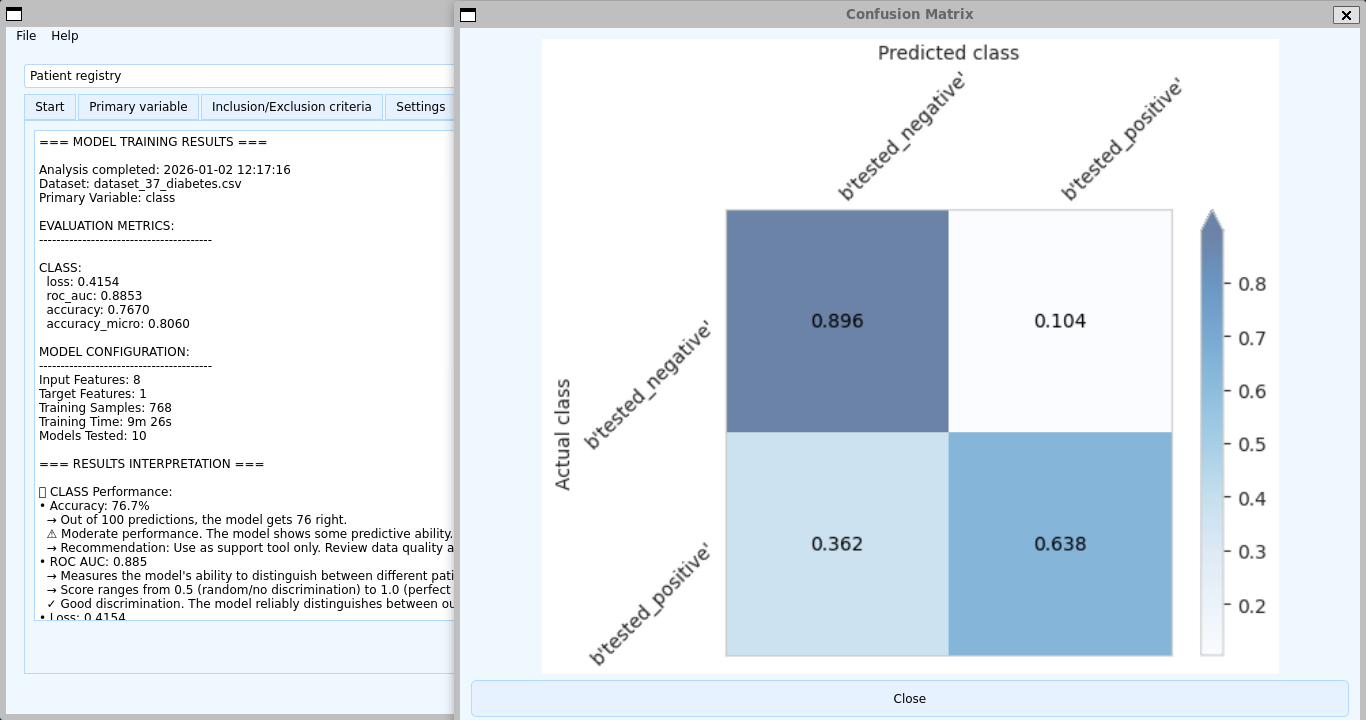
\includegraphics[width=0.8\textwidth]{img/Interface/interface-confusionmatrix.png}
    \end{figure}
\end{frame}

\begin{frame}{Protocol-Aware Interaction Mechanisms}
    \begin{itemize}
        \item \textbf{Variable classification}:\\
        Demographics, clinical measurements, exposures, outcomes, inclusion/exclusion criteria\\
        Prevents inappropriate use (e.g., inclusion criteria as predictors)
        
        \item \textbf{Temporal phase assignment}:\\
        Define protocol phases, assign variables to phases\\
        Prevents data leakage
        
        \item \textbf{Missing data strategies (9 options)}:\\
        \texttt{fill\_with\_const}, \texttt{fill\_with\_mode}, \texttt{fill\_with\_mean}, \texttt{fill\_with\_false}\\
        \texttt{bfill} (backward fill), \texttt{ffill} (forward fill), \texttt{drop\_row}\\
        Default for target: \texttt{drop\_row}
        
        \item \textbf{Custom evaluation metrics}:\\
        Classification: accuracy, precision, recall, F1, AUC-ROC\\
        Regression: MAE, RMSE, $R^2$\\
        User specifies optimization metric
        
        \item \textbf{Interpretable visualizations}:\\
        Confusion matrix heatmap, performance comparison charts
    \end{itemize}
\end{frame}


% Sección: Conclusions
\section{Conclusions}

\begin{frame}{Conclusions and Future Work}
    \begin{block}{Main Contributions}
        \begin{itemize}
            \item \textbf{First end-to-end HGML system} designed specifically for clinical research
            \item \textbf{Protocol-aware interface} supporting CRP competencies (temporal structure, inclusion/exclusion logic, clinical missing data strategies)
            \item \textbf{HCAI-compliant design} achieving high automation + high human control
            \item \textbf{Ready-to-use software} for non-AI specialists
        \end{itemize}
    \end{block}
    
    \begin{block}{Future Work}
        \begin{itemize}
            \item \textbf{User evaluation}: Usability testing with CRPs on real clinical studies
            \item \textbf{Feature completion}: Recruitment timeline, Table 1 generation, univariate distributions
            \item \textbf{Advanced interpretability}: SHAP values, partial dependence plots
            \item \textbf{Regulatory compliance}: Audit trails, model documentation for ethical review
            \item \textbf{Multi-center support}: Leave-one-site-out validation, federated learning
        \end{itemize}
    \end{block}
\end{frame}


% Slide (frame) del título
\begin{frame}
    \titlepage
\end{frame}

\end{document}